\section{Appendix}

\subsection{Logging Table}
\label{subsection:appendixLogging}

\begin{tabu} to 0.8\textwidth { | X[l] | X[c] | }
 \hline
 Timestamp & Date and time of log entry. \\
 \hline
 Condition  & Condition of avatar:weak (c3), average (c2), strong (c1).   \\
\hline
 SplashScreen  & State of black screen     \\
\hline
 HeadX  & item 22    \\
\hline
 HeadY  & item 22    \\
\hline
 HeadZ  & item 22    \\
\hline
 HeadRX  & item 22    \\
\hline
 HeadRY  & item 22    \\
\hline
 HeadRZ  & item 22    \\
\hline
 RightHandx  & item 22    \\
\hline
 RightHandy  & item 22    \\
\hline
 RightHandz  & item 22    \\
\hline
 RightHandRX  & item 22    \\
\hline
 RightHandRY  & item 22    \\
\hline
 RightHandRZ  & item 22    \\
\hline
LeftHandx  & item 22    \\
\hline
 LeftHandy  & item 22    \\
\hline
 LeftHandz  & item 22    \\
\hline
 LeftHandRX  & item 22    \\
\hline
 LeftHandRY  & item 22    \\
\hline
 LeftHandRZ  & item 22    \\
\hline
 Action  & item 22    \\
\hline
 GazeTarget  & item 22    \\
\hline
\end{tabu}

\subsection{Instruction Sheet}
\label{subsection:instructionSheet}
\textbf{Instruction sheet for experimenter for VR games study}\\
\\
\textbf{1. Describe the games to users at arrival}\\
We made 2 virtual reality games - a virtual reality tug-of-war game and a whack-a-mole game!
We are interested in providing users with the best gaming VR experience and we need your feedback for the games we designed.\\
\\
Tug of war, if you have not played it, is a game in which you pull a rope with an opponent and the one that pulls stronger wins! For whack a mole you see a mole come up and you have to slap it with your right hand and hold your hand straight like this [show participant].\\
\\
First, for each game we must calibrate these gloves for your hands and then we can start playing. There will be a screen in front of you and you will have to follow some hand movements. I will walk you through the instructions. \\
\\
We first play tug of war and then 4 minutes of whack a mole! After each game, I will kindly ask you to fill in a short survey about your experience and other design aspects. Before you leave, I will ask you for any feedback or suggested improvements you might have about each game. For full disclosure, our conversations during the experiment will be recorded. All data I record will be transcribed and anonymized. Only I have access to the code.\\
\\
But before you I continue the instructions could you please have a look at these two consent forms. There is a place for your name and signature at the end. I will be here and you can ask me any questions while you read. \\
\\
\textbf{2. Tug-of-War Instructions} \\
For tug of war, your task is to play the game and compete at pulling the rope! You will pull the rope 5 times and you can use both hands for that. You must put your right hand in front of the left hand on the rope and hold it like this [show]. I will give you the rope in your hands once we finish calibrating the gloves. Before I place the gloves on your hands could yoou please fill in this page from the survey with your information [Show participant survey on laptop page and tell them to click next after inputting their data. The next page will not be filled in. Tell them you will shortly explain what that is. After they fill in the questions start putting the gloves on their hands and continue explaining.]\\
\\
In the game you will see your opponent and a countdown will begin. When you see START you should start pulling the rope and keep pulling until you see stop, When you see stop you should stop pulling the rope and the round will be over.\\
\\
After each rope-pull, there will be a set of questions in VR on a panel and I will kindly ask you to read the questions out loud and tell me your answer. I will record your answers in this survey on the laptop, there [show].\\
\\
You have to remember 2 things:
\begin{enumerate}
\itemsep0em 
    \item Try pulling the rope without moving your feet.
    \item Keep your hands on the rope at all times, even when you are reading questions between rope-pulls.
\end{enumerate}
\textbf{3. Setup and runtime instructions} \\
\\
At all times:
\begin{enumerate}
\itemsep0em 
    \item Keep trackers of gloves charged
    \item Keep batteries in charging port
    \item Gloves demagnetized daily/several times per day
    \item Always let participants know what you want to do. (eg.  I will turn off the game now). 
    \item Always let participants know if you want to move them or adjust any parts of the VR setup such as the headset or gloves, especially if it involves touching them. 
\end{enumerate}
Before participant arrival:
\begin{enumerate}
\itemsep0em 
\item Wipe headset
\item Close windows in experiment room
\item Check all devices are tracked
\item Put laptop speakers on the correct output
\item Start survey
\item Adds participant ID and click next
\item Replace batteries on gloves if needed
\item Demagnetize gloves if needed
\item Turn on trackers of gloves
\item Turn on gloves
\item Make sure trackers are synced with steam (they have a green light)
\item Turn on both unity projects
\item Start force meter
\item Turn on camera 
\item Turn on OBS 
\item Make sure Windows picks the correct webcam, the one over the force meter
\item Start Unity and open both games
\item Place Camera and Unity Game view side by side to capture them with OBS.
\end{enumerate}
At start experiment
\begin{enumerate}
\itemsep0em 
\item Greet participant.
\item Explain intro story
\item Give participant both consent forms to sign
\item Participant is invited to complete data with gender and age
\item Do you have any questions? You can ask me anything throughout the experiment.
\item Give participants gloves
\item Give participant headset protector
\item Give participants headset
\item Do glove calibration
\item Tell participants you will give them the rope in their hands now
\item Give participant rope in hands 
\item Tell them to grab the rope with right hand in front of left
\item Tell participant First I will show you the VR setup. I would like you to look around for a minute, tell me if everything is clear, if you can see your hands, the rope, and if the words on the panel are clear.
\item Start PreTrial scene.
\item Stop scene.
\item START FORCE METER (if it turned off)
\item START RECORDING OBS
\item START RECORDING CAMERA
\item START GAME in Experiment scene
\item  Tell participant: \textit{Now I will start the game and you will be facing your opponents. Remember to start pulling when you see START and stop pulling when you see stop. Don’t forget, always keep your hands on the rope.}
\item Remind participants of constraints at trial 3
\item At 4th rope pull, tell participant there are 2 more rounds.
\item For question-answering, tell participant whenever you are ready to take their answers and after each answer tell them some word of acknowledgement that you got their answer (eg. ok, Alright). Refrain from using overly positive adjectives like great, to prevent encouraging them to give positive answers.
\end{enumerate}
\textbf{4. End instructions}\\
\textit{Note that the experiment instructions for the whack-a-mole game are nor presented as they are out of the scope for this research. Participants always played tug-of-war first, completed its related survey, then played whack-a-mole and completed its related survey.}\\
\\
Take a pen, paper and write participant feedback during the interview.
\begin{enumerate}
\itemsep0em
\item Thank the participant.
\item  I would like to ask you now if you have any suggestions to improve the first game, the tug-of-war game? What was your impression?
\item What about the whack-a-mole game? Do you have any thoughts about that game?
\item Thank you for the feedback. One last question before you go. Could explain to me, in your own words what this experiment was about? Based on what you saw and what I explained.
\end{enumerate}
At the end of each day do the logging:
\begin{enumerate}
\itemsep0em
    \item Log participant feedback in document on Google Drive.
    \item Move logs in experiment folder for both games and commit to Git.
    \item Rename recorded videos with participant id and upload them to Google Drive.
\end{enumerate}
\subsection{Consent form}
\label{subsection:consentForm}
\textbf{Informed Consent Form for Volunteer Participants}
This informed consent form is for volunteer participants to take part in an experiment about playing tug of war in virtual reality with different players. This research is done by a student following a master’s degree in Computer Science at the University of Copenhagen, Denmark as part of their Master Thesis. This research is under the supervision of professors Henning Pohl and Kasper Hornbæk from the University of Copenhagen.\\
\\
This Informed Consent Form has two parts:
\begin{itemize}
    \item  Information Sheet (to share information about the research with you, the volunteer participant)
    \item  Certificate of Consent (for giving your consent if you agree to take part)
\end{itemize}
\textbf{PART I: Information Sheet}
\textbf{Introduction}
I am Andreea-Anamaria Muresan, a student at the University of Copenhagen, and I am doing a master thesis about interactions in virtual reality.\\
\\
I would like to invite you to be part of this research. In this document, you can find detailed information about the project. Before you decide, you can talk to anyone you feel comfortable with about the research. If there are words that you do not understand please ask me about them and I will take time to explain. If you have questions later, you can ask me or even pose your query to the project supervisors.\\
\\
\textbf{Purpose of the research and type of manipulation}
The purpose of this research is to evaluate a rope-pulling game in virtual reality. In this evaluation, we look at the quality of the virtual rope, the design of the players and measure body ownership and presence in the virtual world.\\
\\
\textbf{Participant selection}
You have been invited to this study because you satisfy the following requirements: you are representative of a group of users who may use virtual reality.\\
\\
\textbf{Voluntary Participation}\\
Your participation in this research is entirely voluntary. It is your choice whether to participate or not. You can change your mind later and stop participating even if you agreed earlier.\\
\\
\textbf{Procedures and Protocol}\\
Throughout this experiment you will be asked to:
\begin{enumerate}
\itemsep0em 
    \item Play tug-of-war,
    \item Complete a verbal questionnaire after each rope-pull, 
    \item  Fill in a survey after finishing the game,
    \item  Have a short chat before you leave and tell us your opinion about the game and how we can improve it. Our conversations will be recorded and anonymized. 
\end{enumerate}
At the beginning of each round, you will hear and see a countdown. You must start pulling when you see \textbf{Start} and you must stop pulling once you see \textbf{Stop}. \\
Please try to:
\begin{enumerate}
\itemsep0em
    \item Grab the rope with your right hand in front of the left hand.
  \item Keep your hands on the rope at all times. 
  \item Do not move your hands on the rope once you grab it.
  \item Try pulling the rope with your upper body and arms. Try keeping your feet in the same starting position.
\end{enumerate}
\textbf{Duration}\\
The experiment is expected to last between 20 and 30 minutes. \\
\\
\textbf{Risks and Benefits}\\
We anticipate no risks from participating in the experiment. If you participate in the experiment you will help the student conducting the experiment complete their Master Thesis successfully as well as gain experience running, designing experiments and interacting with participants.\\
\\
\textbf{Reimbursements}
You will not be given any money or gifts to take part in this research.\\
\\
\textbf{Confidentiality}\\
The data we collect from you will be made anonymous; your name will be replaced with a number known only to the person running and designing the experiment.\\
\\
\textbf{Sharing the Results}\\
If you are interested, you may leave us your email or contact us at a later stage to learn about the outcomes of the study. No confidential information will be shared.\\
\\
\textbf{Right to Refuse or Withdraw}\\
You do not have to take part in this research if you do not wish to do so. You may also stop participating in the research at any time you choose. It is your choice and all your rights will be respected.\\
\\
\textbf{Who to Contact}\\
If you have any questions about the study at a later stage, please contact the student investigator at the following email addresses: 
Andreea-Anamaria Muresan: zph748@alumni.ku.dk\\
You can ask me any questions about any part of the research study if you wish. Do you have any questions so far?\\
\\
\textbf{PART II: Certificate of Consent}\\
I have read the foregoing information. I have had the opportunity to ask questions about it and any questions that I asked have been answered to my satisfaction. Below I mark that I consent voluntarily to participate as a participant in this research. \\
Print Name of Participant: \\
Signature of Participant: \\
Date (Day/Month/Year):    \\
\\
\textbf{Statement by the researcher/person taking consent}\\
I confirm that the participant was given an opportunity to ask questions about the study, and all the questions asked by the participant have been answered correctly and to the best of my ability. I confirm that the individual has not been coerced into giving consent, and the consent has been given freely and voluntarily.\\
Print Name of person taking the consent:  \\ 
Signature of person taking the consent:  \\   
Date (Day/Month/Year):              \\            	
\subsection{Coding Tables}
\label{subsubsection:codingTables}
\begin{table}[H]
\begin{minipage}{.5\linewidth}
\centering
\begin{tabu}  { | p{1cm}| p{2cm}| p{2cm} | }
\hline
\textbf{ID} & \textbf{Name} & \textbf{Condition}\\
\hline
1 & F5\_C3 & Weak\\
\hline
2 & F4\_C1 & Strong\\
\hline
3 & F1\_C2 & Average\\
\hline
4 & F6\_C1 & Strong\\
\hline
5 & F1\_C1 & Strong\\
\hline
6 & F3\_C1 & Strong\\
\hline
7 & F5\_C1 & Strong\\
\hline
8 & F5\_C2 & Average\\
\hline
9 & F1\_C3 & Weak\\
\hline
10 & F4\_C3 & Weak\\
\hline
11 & F2\_C3 & Weak\\
\hline
12 & F6\_C2 & Average\\
\hline
13 & F6\_C3 & Weak\\
\hline
14 & F4\_C2 & Average\\
\hline
15 & F3\_C3 & Weak    \\
\hline
16 & F2\_C2 & Average\\
\hline
17 & F2\_C1 & Strong\\
\hline
18 & F3\_C2 & Average\\
\hline
\end{tabu}
\caption{Female avatar designs coding.}
\label{table:codingFemales}
\end{minipage}
\begin{minipage}{.5\linewidth}
\centering
\begin{tabu} { | p{1cm}| p{2cm}| p{2cm} | }
\hline
\textbf{ID} & \textbf{Name} & \textbf{Condition}\\
\hline
1 & M6\_C3 & Weak\\
\hline
2 & M5\_C1 & Strong\\
\hline
3 & M1\_C2 &  Average\\
\hline
4 & M7\_C1 &Strong \\
\hline
5 & M1\_C1 & Strong \\
\hline
6& M3\_C1 & Strong\\
\hline
7& M6\_C1 & Strong \\
\hline
8& M6\_C2 & Average \\
\hline
9& M1\_C3 & Weak \\
\hline
10& M5\_C3 & Weak \\
\hline
11& M2\_C3 & Weak \\
\hline
12& M7\_C2 & Average\\
\hline
13& M7\_C3 & Weak \\
\hline
14& M5\_C2 & Average \\
\hline
15& M3\_C3 & Weak \\
\hline
16& M2\_C2 & Average\\
\hline
17& M2\_C1 & Strong\\
\hline
18 & M3\_C2 & Average\\
\hline
\end{tabu}
\caption{Male avatar designs coding.}
\label{table:codingMales}
\end{minipage}
\end{table}
\subsection{Survey Mean Ratings}
\label{subsection:MeanRatings}
\begin{table}[H]
    \centering
    \addtolength{\leftskip} {-2cm}
    \addtolength{\rightskip}{-2cm}
    \begin{tabu}{|c|c|c|c|c|c|c|}
     \hline
        \textbf{ID} & \textbf{Attractive} &\textbf{Intelligent} &\textbf{Intimidating}
        &\textbf{Strong} &\textbf{Weighted} &\textbf{UMA}\\
        \hline
10	& 1.93333 &	2.66667	& 1.66667 &	1.46667 &	1.56667 &	f4 c3\\
\hline
15 &	1.73334 &	2.46667 &	1.73334 &	1.53334	& 1.63334 &  \\
\hline
14 & 1.93334 & 2.8	& 2 & 1.4666 & 1.73333  & \\
\hline
8	& 2.46667	& 2.8	& 1.8 &	1.86667	& 1.83333 & 	\\
\hline
11 & 2.33333 &3& 1.6 &2.06667 & 1.83333 & \\
\hline
16&	2.86667 &	3&	1.73333	&2.06667 &	1.9 &	f2 c2\\
\hline
9 &1.8	& 2.6 &	2.2	&1.66667	 & 1.93333 & 	\\
\hline
13	& 2.06667	& 2.66667 & 1.93333 & 1.93333&	
1.93333 & \\	
\hline
1 &2&	2.33333	&1.86667	&2.06667	& 1.96667	&\\
\hline
18 &	2.26667	 & 2.6 &	2.2&	2	& 2.1	&f3 c2\\
\hline
12&	2.4	&2.66667&	2.06667&	2.26667&	2.16667 &\\
\hline
7 &	1.8 &	2.13333&	2.13333&	2.33333&	2.23333 &\\
\hline
3&2&	2.8&	2.66667&	2.66667&	2.66667	& \\
\hline
5 & 1.53333 & 2.2	& 2.73333	& 3	& 2.86667 &	f1 c1 \\
\hline
17	& 1.6	& 2.2 &	2.86667	& 3.06667 &	2.96667 & \\
\hline
4	&1.73333	&2.33333&	3	&3.26667&	3.13333 &	\\
\hline
6	&1.66667&	2.4	&2.73333	&3.53333	& 3.13333 &\\
\hline
2	&1.46667	&2.2	&3.4	&3.46667	&3.43333	&F4 c1\\
\hline
    \end{tabu}

    \caption{Female mean ratings.}
    \label{tab:f_mean}
    \begin{tabu}{|c|c|c|c|c|c|c|}
     \hline
        \textbf{ID} & \textbf{Attractive} &\textbf{Intelligent} &\textbf{Intimidating}
        &\textbf{Strong} &\textbf{Weighted} &\textbf{UMA}\\
        \hline
13	&2.625	&3.0625	&1.25&	1.25&	1.25&	m7 c3 \\
\hline
8	&2.5&	2.6875	&1.5625&	1.875&	1.71875&	\\
\hline
1&	2.1875&	2.4375	&2.125&	1.375&	1.75& \\
\hline
9&	1.25&	1.625&	2.125&	1.75	&1.9375&	\\
\hline
12&	3.5	&3.3125	&1.5625&	2.375	&1.96875&	m7 c2\\
\hline
11&	1.8125&	2.3125&	2&	2.25&	2.125& \\
\hline
15	&1.8125	&2.1875	&2.125&	2.5625&	2.34375&	\\
\hline
10&	2&	2.375&	2.3125&	2.4375&	2.375&	\\
\hline
7&	1.75&	2.8125	&2.3125&	2.75&	2.53125&	m6 c1\\
\hline
4&	2.375&	2.5625&	2.3125&	3.3125&	2.8125&	\\
\hline
16&	2.0625&	2.25&	2.375&	3.3125&	2.84375	& \\
\hline
18	&2.625&	2.625&	2.5625&	3.5625&	3.0625&	 \\
\hline
14&	2.3125&	2.5	&2.75	&3.5625	&3.15625&	\\
\hline
3&	1.375	&1.9375&	3.5&	3.0625&	3.28125	&m1 c2\\
\hline
6&	2.5625&	2.5625&	3.0625&	4.1875&	3.625&	\\
\hline
5&	1.5625&	2.3125&	3.5625&	4.0625	&3.8125& \\
\hline
17	&2.25&	2.125&	3.625&	4.6875&	4.15625	&\\
\hline
2&	1.9375&	2&	3.8125&	4.75&	4.28125&	m5  c1\\ 
\hline
    \end{tabu}
    \caption{Male mean ratings.}
    \label{tab:m_mean}
\end{table}
\subsection{Survey Thumbnails and Ratings}
\label{subsection:thumbnails}
\subsubsection{Females}
\begin{figure}[H]
\minipage{0.5\textwidth}
  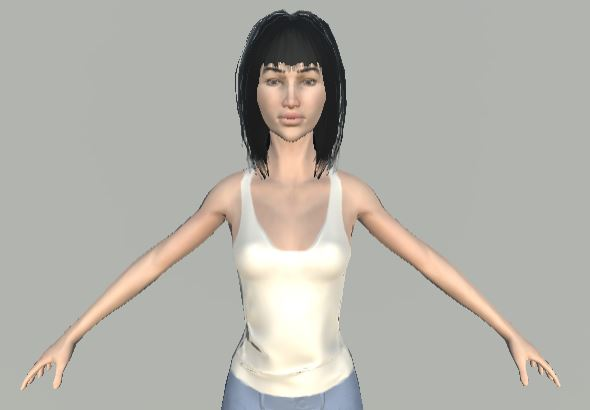
\includegraphics[width=\linewidth]{Images/Females/1.JPG}
\endminipage\hfill
\minipage{0.5\textwidth}
  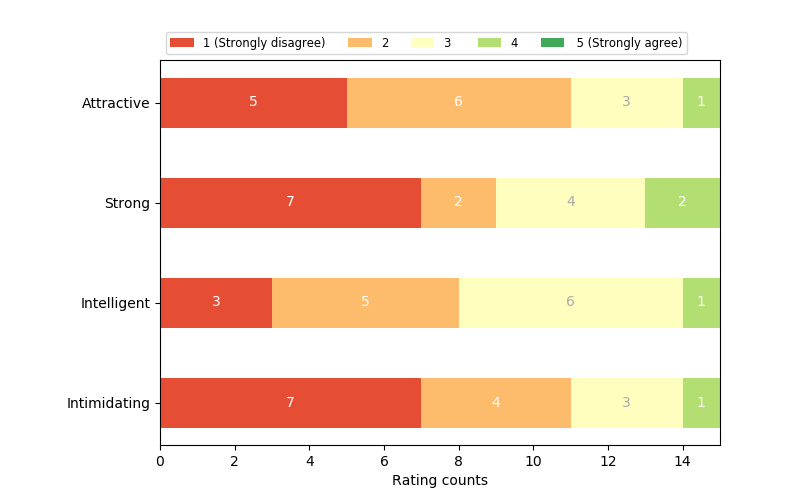
\includegraphics[width=\linewidth]{Survey/FRatings/avatar_f1.png}
\endminipage\hfill
\caption{Female 1 thumbnail and ratings.}
\end{figure}

\begin{figure}[H]
\minipage{0.5\textwidth}
  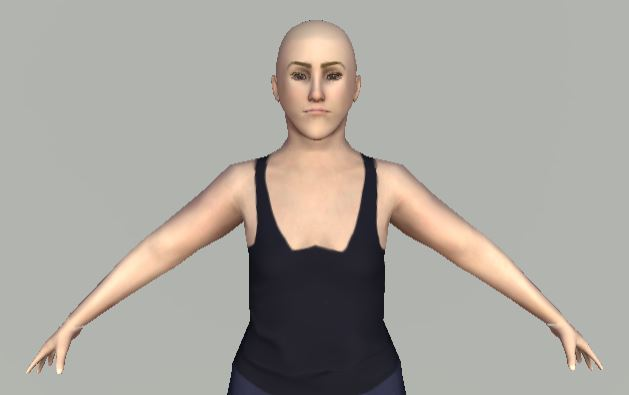
\includegraphics[width=\linewidth]{Images/Females/2.JPG}
\endminipage\hfill
\minipage{0.5\textwidth}
  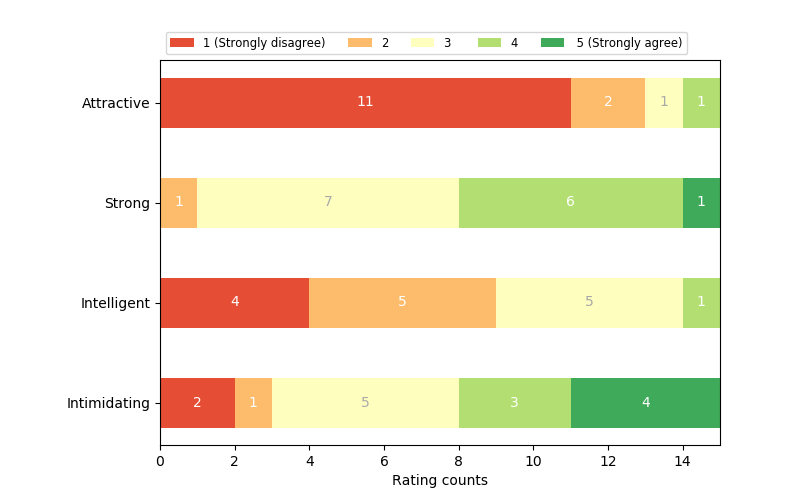
\includegraphics[width=\linewidth]{Survey/FRatings/avatar_f2.png}
\endminipage\hfill
\caption{Female 2 thumbnail and ratings.}
\end{figure}

\begin{figure}[H]
\minipage{0.5\textwidth}
  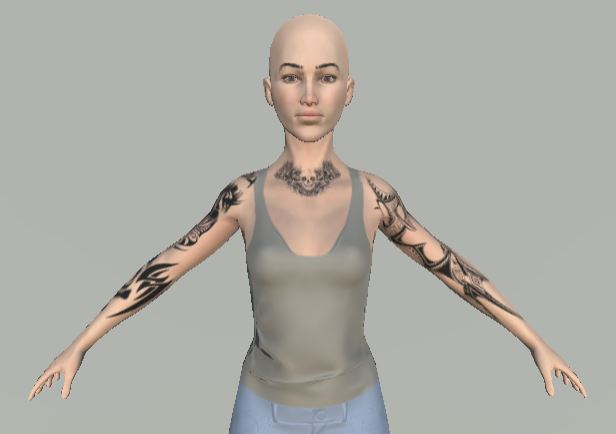
\includegraphics[width=\linewidth]{Images/Females/3.JPG}
\endminipage\hfill
\minipage{0.5\textwidth}
  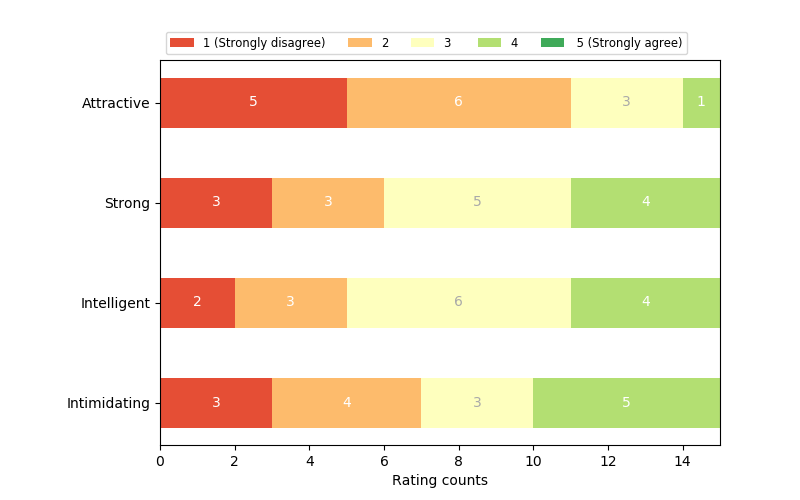
\includegraphics[width=\linewidth]{Survey/FRatings/avatar_f3.png}
\endminipage\hfill
\caption{Female 3 thumbnail and ratings.}
\end{figure}

\begin{figure}[H]
\minipage{0.5\textwidth}
  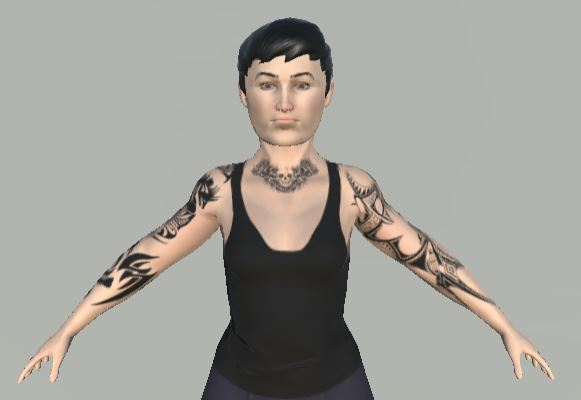
\includegraphics[width=\linewidth]{Images/Females/4.JPG}
\endminipage\hfill
\minipage{0.5\textwidth}
  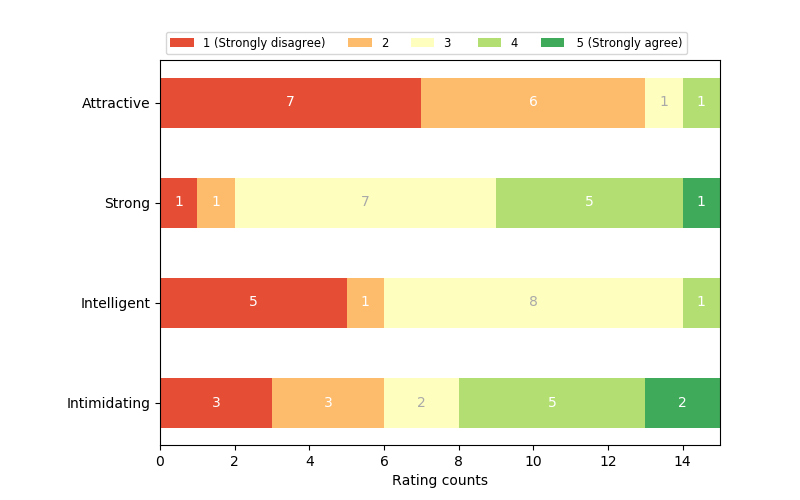
\includegraphics[width=\linewidth]{Survey/FRatings/avatar_f4.png}
\endminipage\hfill
\caption{Female 4 thumbnail and ratings.}
\end{figure}

\begin{figure}[H]
\minipage{0.5\textwidth}
  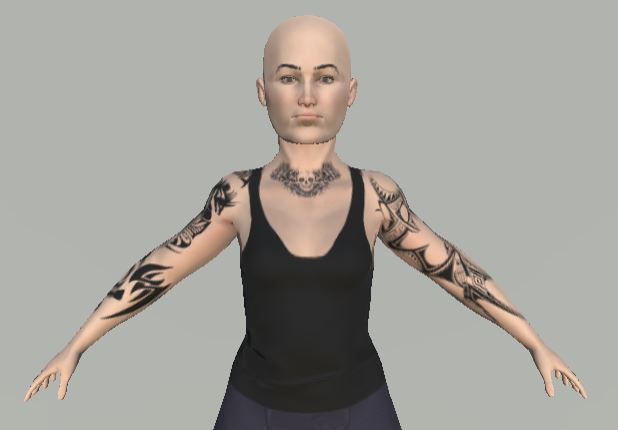
\includegraphics[width=\linewidth]{Images/Females/5.JPG}
\endminipage\hfill
\minipage{0.5\textwidth}
  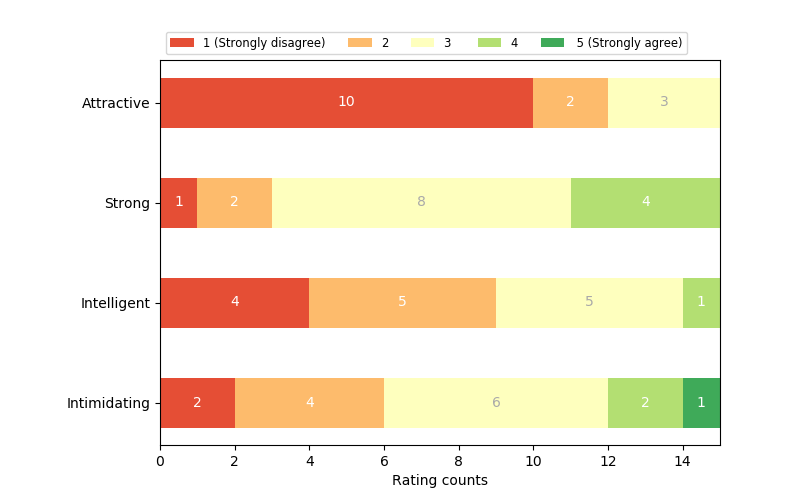
\includegraphics[width=\linewidth]{Survey/FRatings/avatar_f5.png}
\endminipage\hfill
\caption{Female 5 thumbnail and ratings.}
\end{figure}

\begin{figure}[H]
\minipage{0.5\textwidth}
  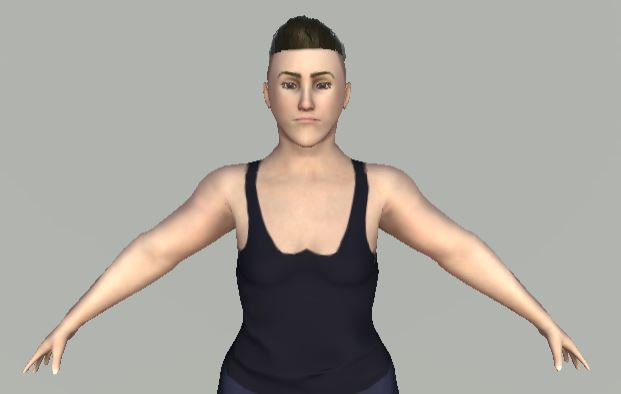
\includegraphics[width=\linewidth]{Images/Females/6.JPG}
\endminipage\hfill
\minipage{0.5\textwidth}
  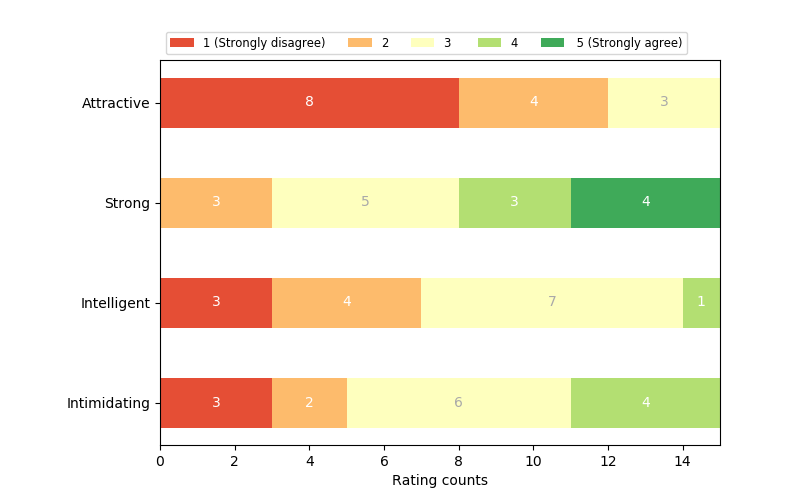
\includegraphics[width=\linewidth]{Survey/FRatings/avatar_f6.png}
\endminipage\hfill
\caption{Female 6 thumbnail and ratings.}
\end{figure}


\begin{figure}[H]
\minipage{0.5\textwidth}
  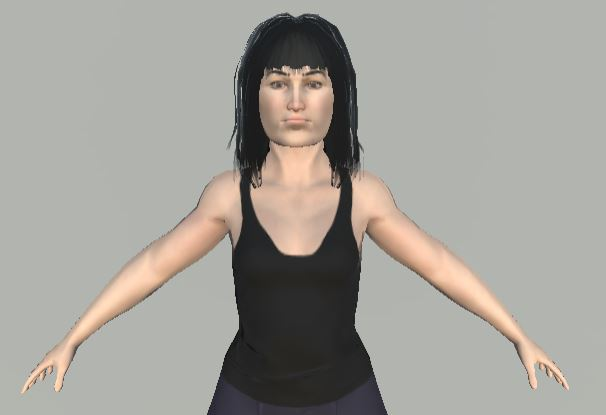
\includegraphics[width=\linewidth]{Images/Females/7.JPG}
\endminipage\hfill
\minipage{0.5\textwidth}
  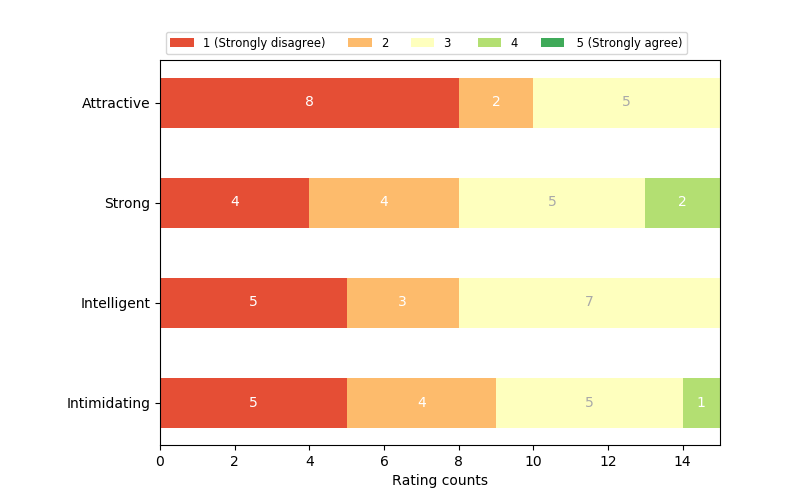
\includegraphics[width=\linewidth]{Survey/FRatings/avatar_f7.png}
\endminipage\hfill
\caption{Female 7 thumbnail and ratings.}
\end{figure}


\begin{figure}[H]
\minipage{0.5\textwidth}
  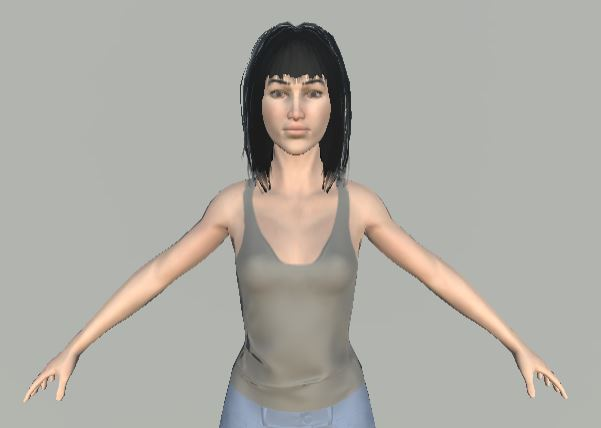
\includegraphics[width=\linewidth]{Images/Females/8.JPG}
\endminipage\hfill
\minipage{0.5\textwidth}
  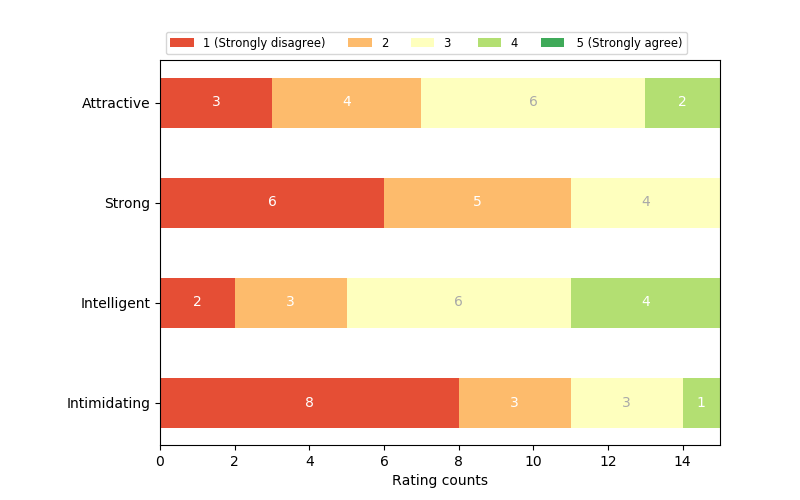
\includegraphics[width=\linewidth]{Survey/FRatings/avatar_f8.png}
\endminipage\hfill
\caption{Female 8 thumbnail and ratings.}
\end{figure}


\begin{figure}[H]
\minipage{0.5\textwidth}
  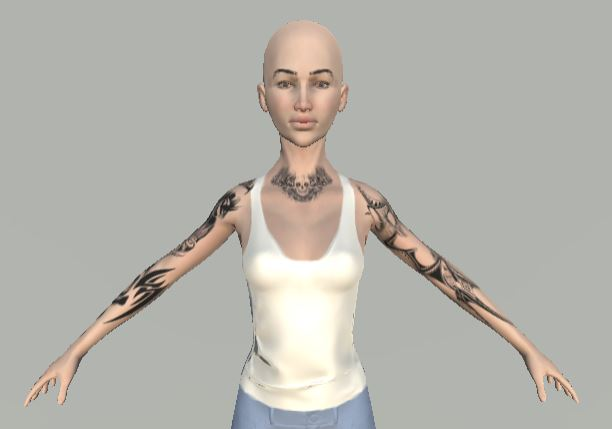
\includegraphics[width=\linewidth]{Images/Females/9.JPG}
\endminipage\hfill
\minipage{0.5\textwidth}
  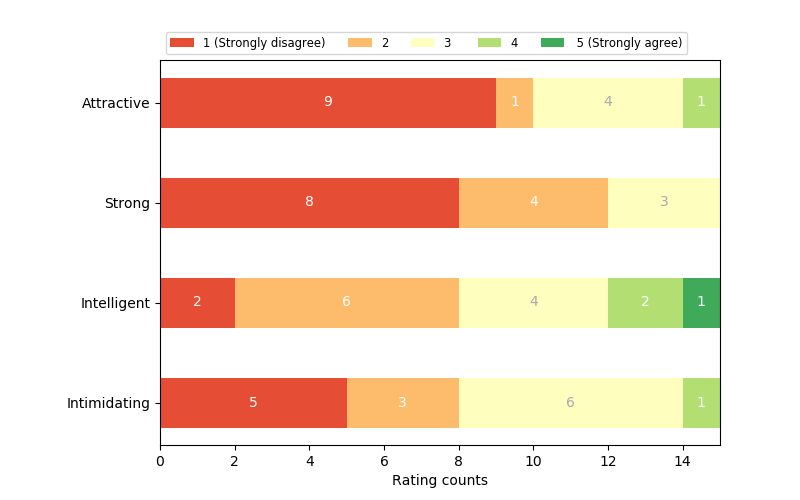
\includegraphics[width=\linewidth]{Survey/FRatings/avatar_f9.png}
\endminipage\hfill
\caption{Female 9 thumbnail and ratings.}
\end{figure}


\begin{figure}[H]
\minipage{0.5\textwidth}
  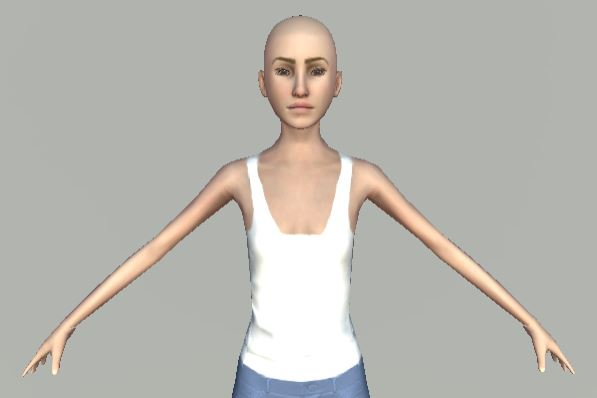
\includegraphics[width=\linewidth]{Images/Females/10.JPG}
\endminipage\hfill
\minipage{0.5\textwidth}
  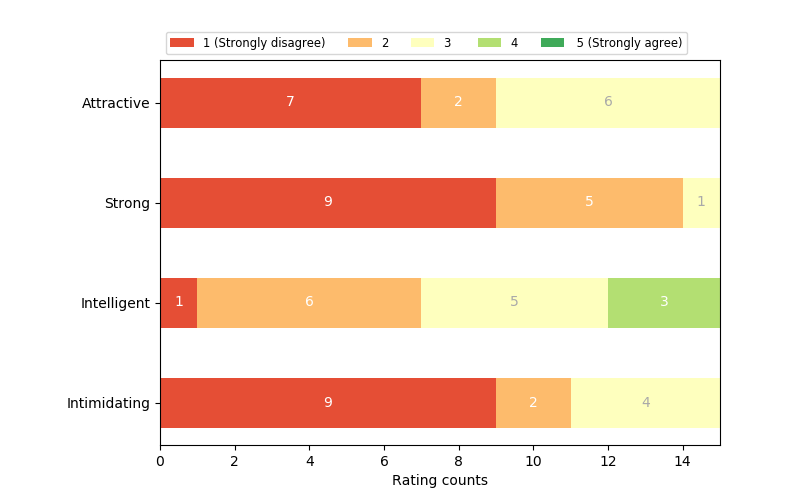
\includegraphics[width=\linewidth]{Survey/FRatings/avatar_f10.png}
\endminipage\hfill
\caption{Female 10 thumbnail and ratings.}
\end{figure}


\begin{figure}[H]
\minipage{0.5\textwidth}
  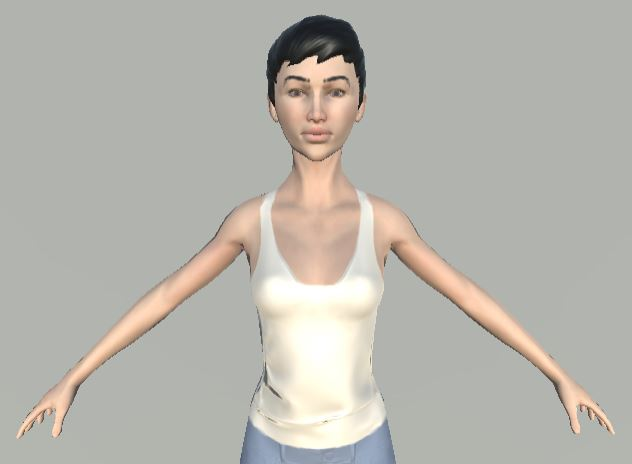
\includegraphics[width=\linewidth]{Images/Females/11.JPG}
\endminipage\hfill
\minipage{0.5\textwidth}
  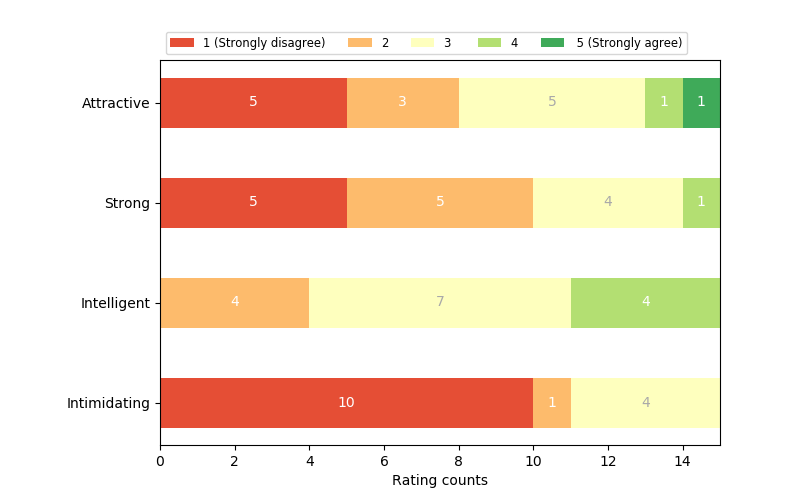
\includegraphics[width=\linewidth]{Survey/FRatings/avatar_f11.png}
\endminipage\hfill
\caption{Female 11 thumbnail and ratings.}
\end{figure}


\begin{figure}[H]
\minipage{0.5\textwidth}
  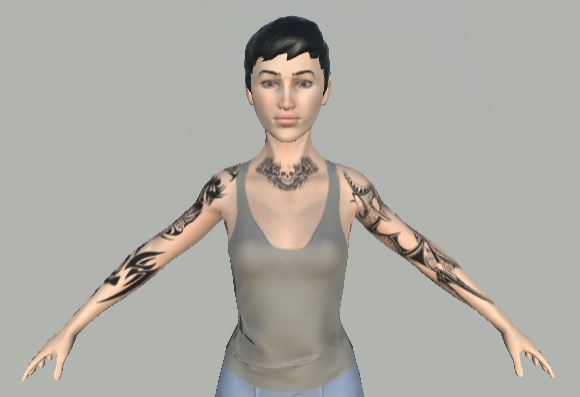
\includegraphics[width=\linewidth]{Images/Females/12.JPG}
\endminipage\hfill
\minipage{0.5\textwidth}
  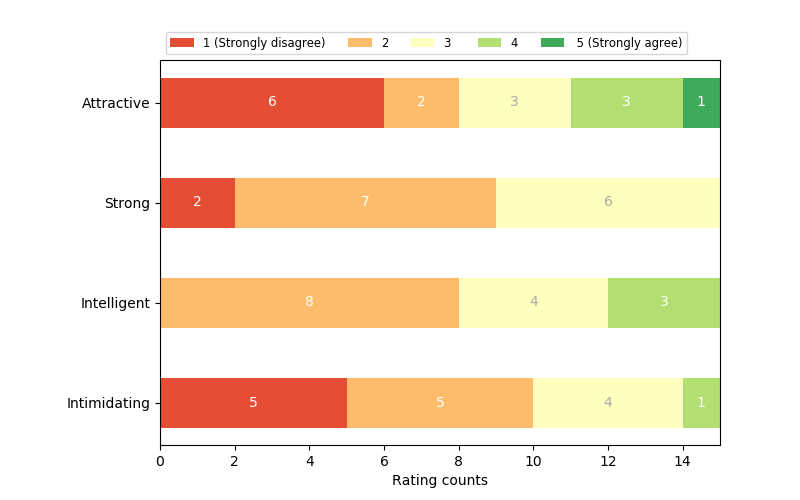
\includegraphics[width=\linewidth]{Survey/FRatings/avatar_f12.png}
\endminipage\hfill
\caption{Female 12 thumbnail and ratings.}
\end{figure}

\begin{figure}[H]
\minipage{0.5\textwidth}
  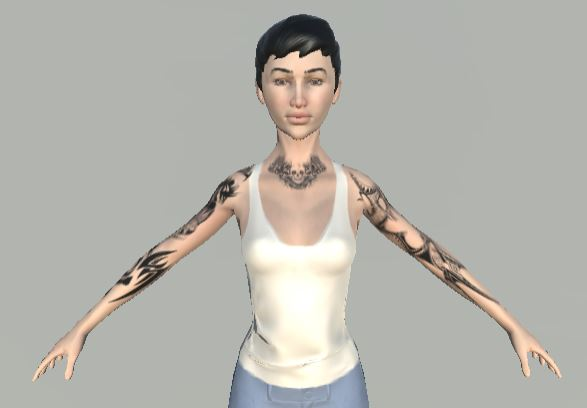
\includegraphics[width=\linewidth]{Images/Females/13.JPG}
\endminipage\hfill
\minipage{0.5\textwidth}
  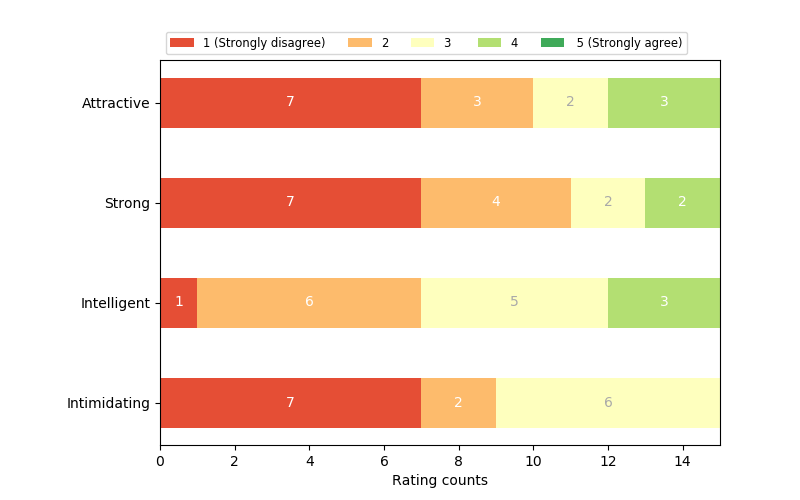
\includegraphics[width=\linewidth]{Survey/FRatings/avatar_f13.png}
\endminipage\hfill
\caption{Female 13 thumbnail and ratings.}
\end{figure}

\begin{figure}[H]
\minipage{0.5\textwidth}
  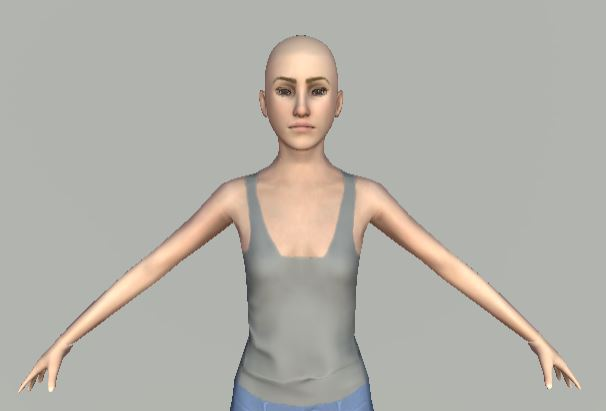
\includegraphics[width=\linewidth]{Images/Females/14.JPG}
\endminipage\hfill
\minipage{0.5\textwidth}
  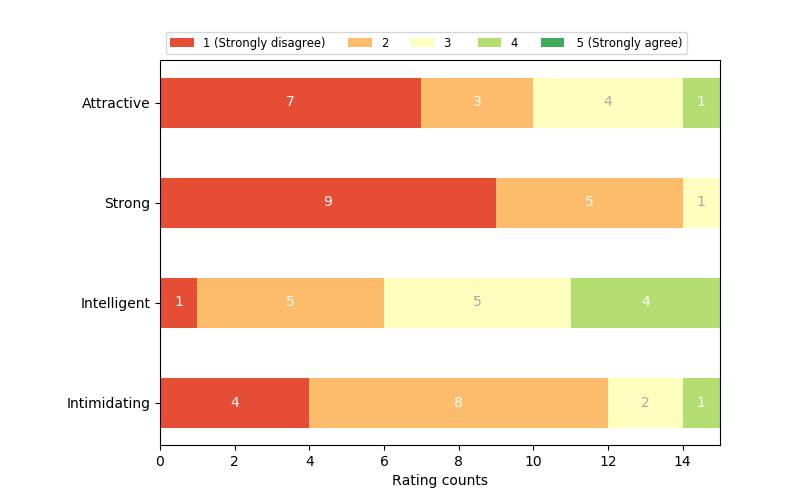
\includegraphics[width=\linewidth]{Survey/FRatings/avatar_f14.png}
\endminipage\hfill
\caption{Female 14 thumbnail and ratings.}
\end{figure}

\begin{figure}[H]
\minipage{0.5\textwidth}
  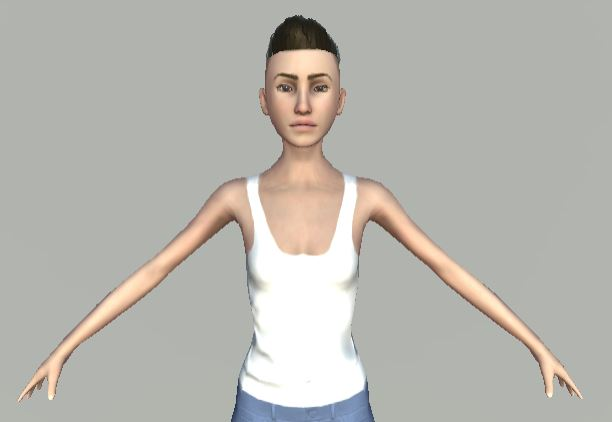
\includegraphics[width=\linewidth]{Images/Females/15.JPG}
\endminipage\hfill
\minipage{0.5\textwidth}
  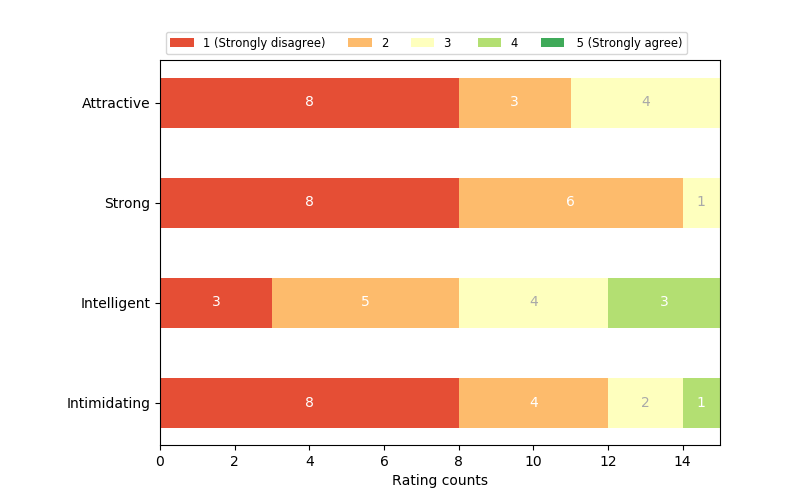
\includegraphics[width=\linewidth]{Survey/FRatings/avatar_f15.png}
\endminipage\hfill
\caption{Female 15 thumbnail and ratings.}
\end{figure}
\begin{figure}[H]
\minipage{0.5\textwidth}
  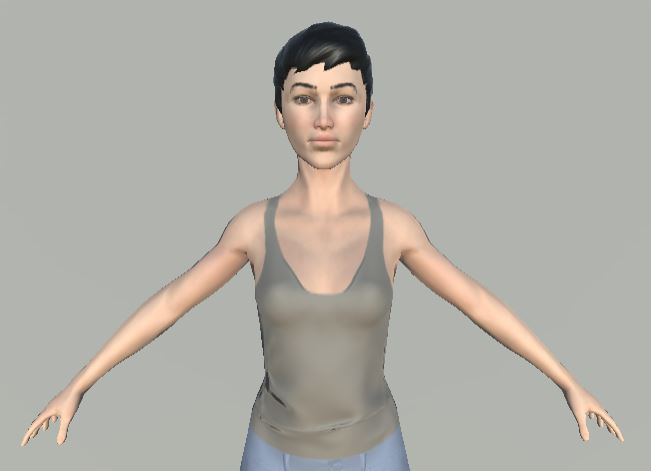
\includegraphics[width=\linewidth]{Images/Females/16.JPG}
\endminipage\hfill
\minipage{0.5\textwidth}
  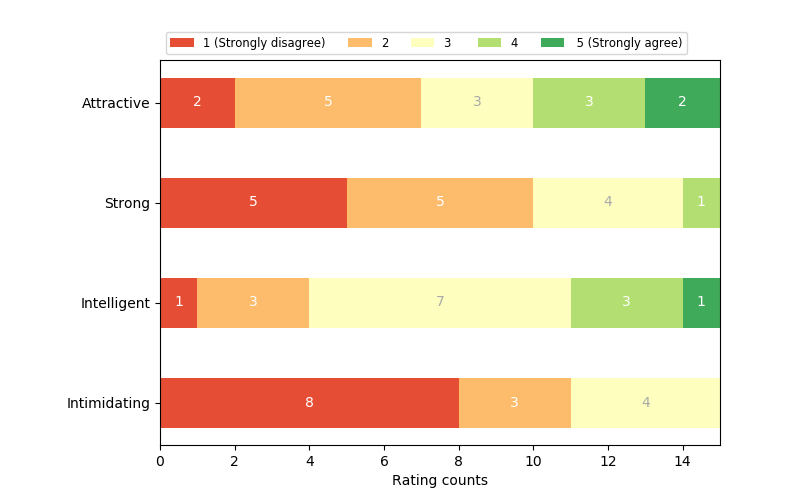
\includegraphics[width=\linewidth]{Survey/FRatings/avatar_f16.png}
\endminipage\hfill
\caption{Female 16 thumbnail and ratings.}
\end{figure}

\begin{figure}[H]
\minipage{0.5\textwidth}
  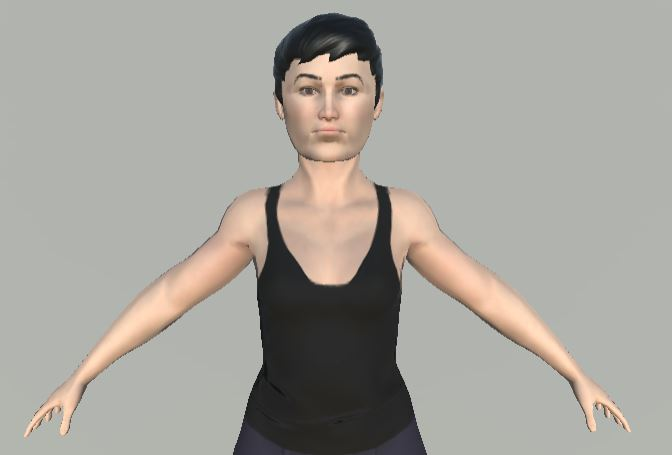
\includegraphics[width=\linewidth]{Images/Females/17.JPG}
\endminipage\hfill
\minipage{0.5\textwidth}
  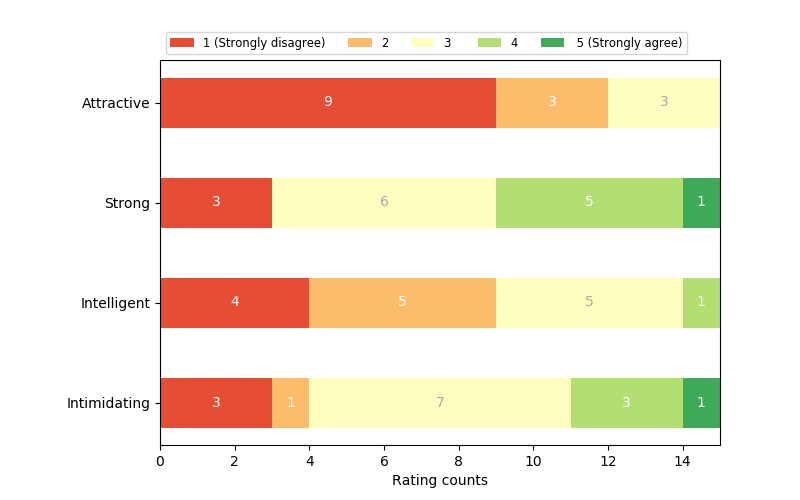
\includegraphics[width=\linewidth]{Survey/FRatings/avatar_f17.png}
\endminipage\hfill
\caption{Female 17 thumbnail and ratings.}
\end{figure}

\begin{figure}[H]
\minipage{0.5\textwidth}
  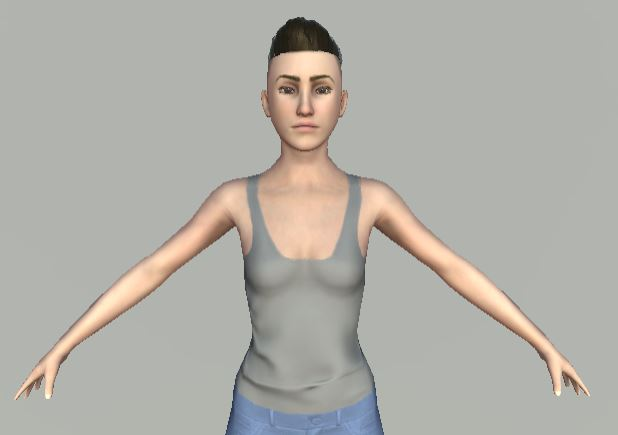
\includegraphics[width=\linewidth]{Images/Females/18.JPG}
\endminipage\hfill
\minipage{0.5\textwidth}
  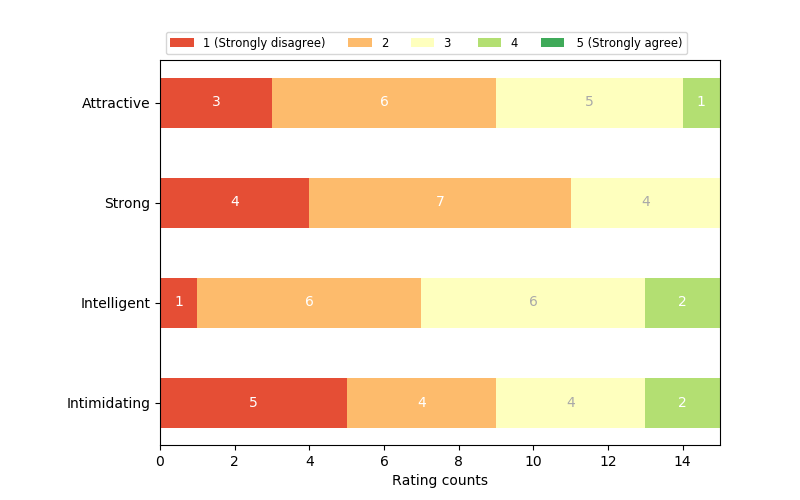
\includegraphics[width=\linewidth]{Survey/FRatings/avatar_f18.png}
\endminipage\hfill
\caption{Female 18 thumbnail and ratings.}
\end{figure}

\subsubsection{Males}

\begin{figure}[H]
\minipage{0.5\textwidth}
  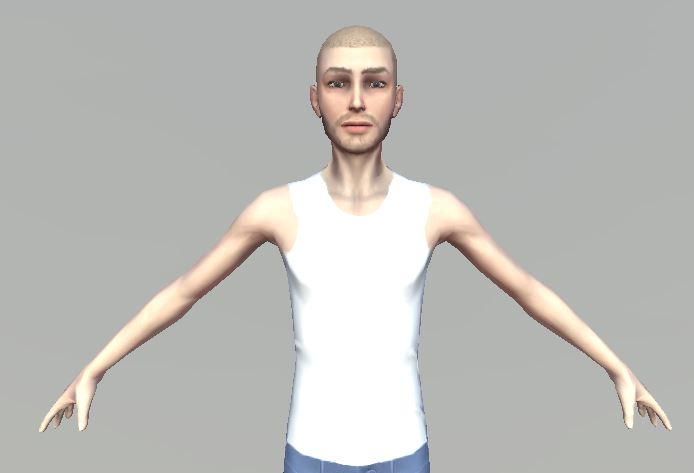
\includegraphics[width=\linewidth]{Images/Males/1.JPG}
\endminipage\hfill
\minipage{0.5\textwidth}
  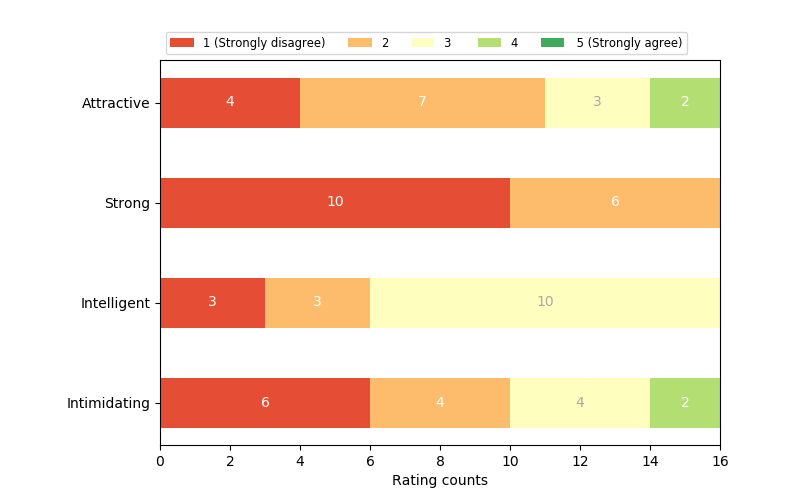
\includegraphics[width=\linewidth]{Survey/MRatings/avatar_m1.png}
\endminipage\hfill
\caption{Male 1 thumbnail and ratings.}
\end{figure}

\begin{figure}[H]
\minipage{0.5\textwidth}
  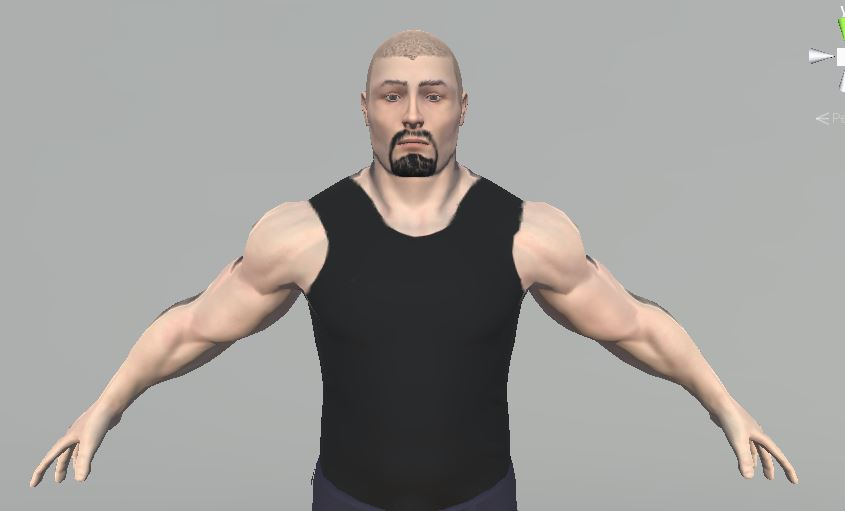
\includegraphics[width=\linewidth]{Images/Males/2.JPG}
\endminipage\hfill
\minipage{0.5\textwidth}
  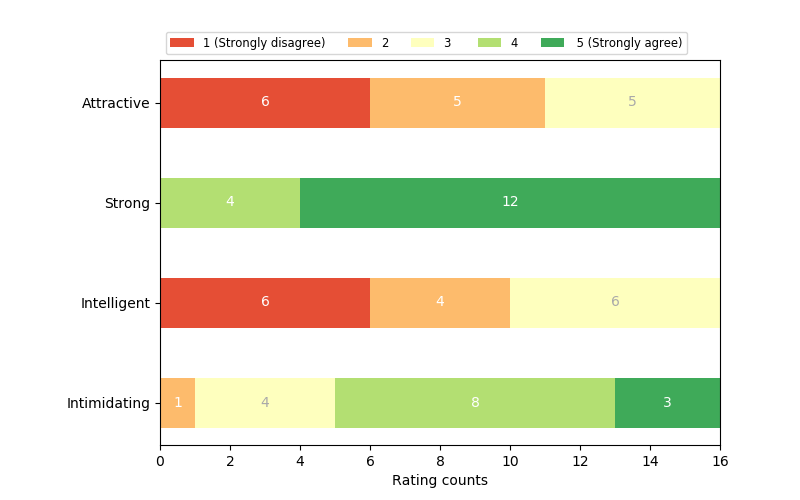
\includegraphics[width=\linewidth]{Survey/MRatings/avatar_m2.png}
\endminipage\hfill
\caption{Male 2 thumbnail and ratings.}
\end{figure}

\begin{figure}[H]
\minipage{0.5\textwidth}
  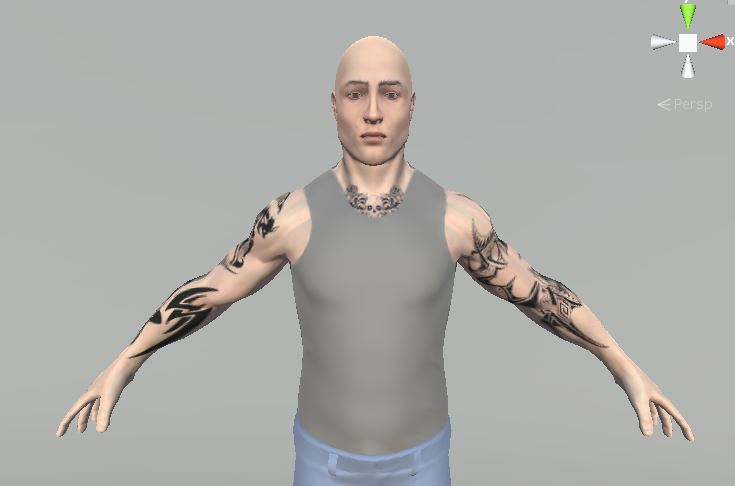
\includegraphics[width=\linewidth]{Images/Males/3.JPG}
\endminipage\hfill
\minipage{0.5\textwidth}
  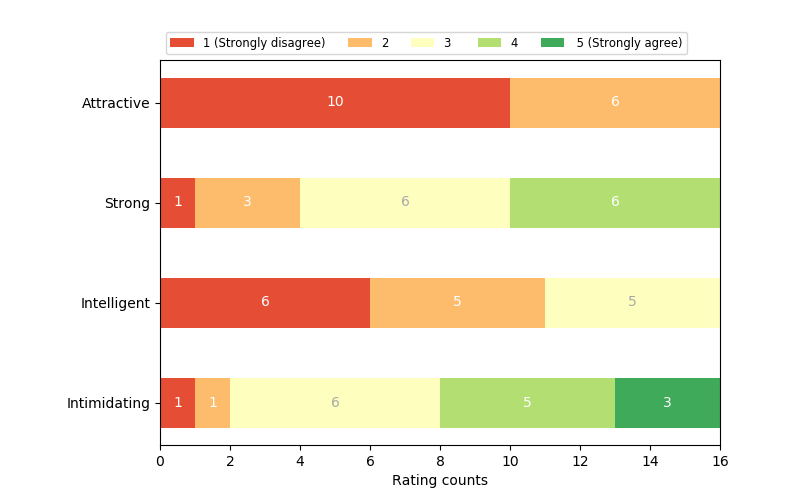
\includegraphics[width=\linewidth]{Survey/MRatings/avatar_m3.png}
\endminipage\hfill
\caption{Male 3 thumbnail and ratings.}
\end{figure}

\begin{figure}[H]
\minipage{0.5\textwidth}
  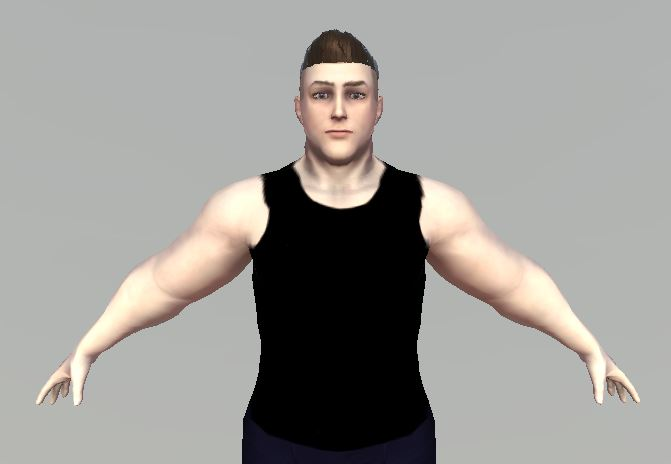
\includegraphics[width=\linewidth]{Images/Males/4.JPG}
\endminipage\hfill
\minipage{0.5\textwidth}
  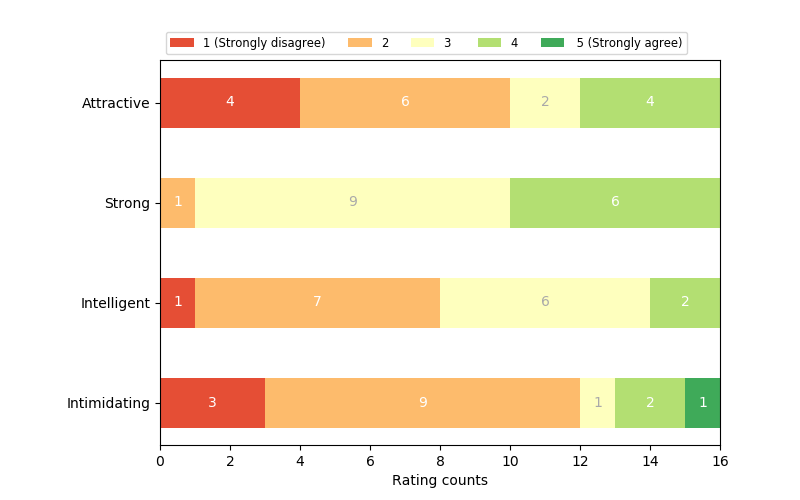
\includegraphics[width=\linewidth]{Survey/MRatings/avatar_m4.png}
\endminipage\hfill
\caption{Male 4 thumbnail and ratings.}
\end{figure}

\begin{figure}[H]
\minipage{0.5\textwidth}
  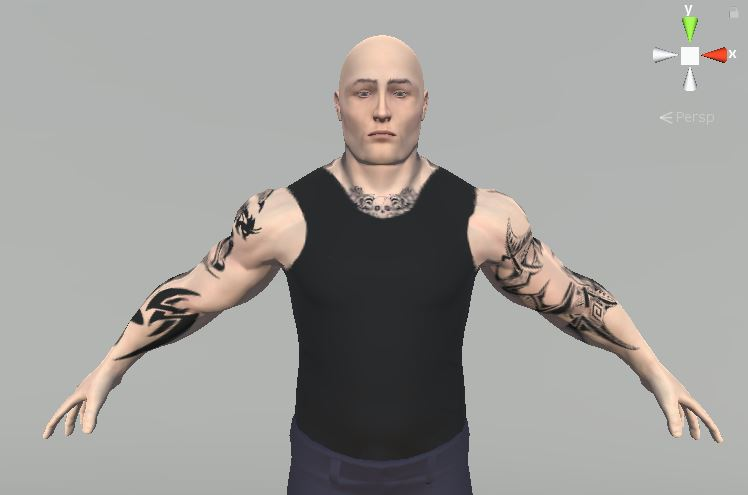
\includegraphics[width=\linewidth]{Images/Males/5.JPG}
\endminipage\hfill
\minipage{0.5\textwidth}
  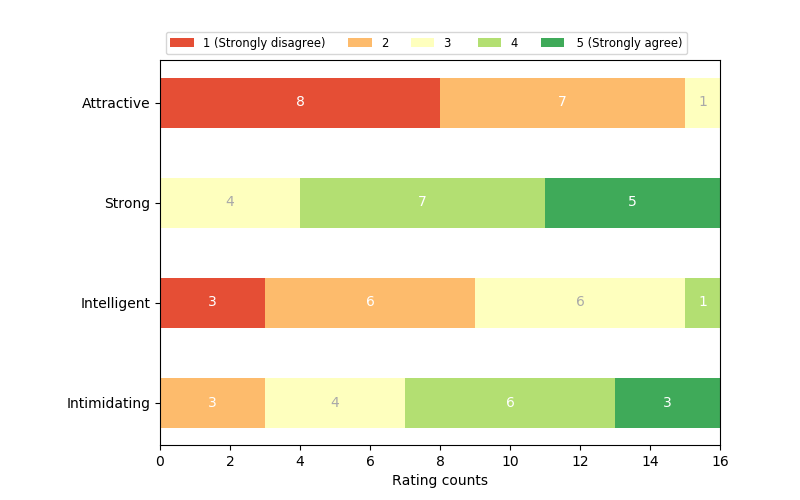
\includegraphics[width=\linewidth]{Survey/MRatings/avatar_m5.png}
\endminipage\hfill
\caption{Male 5 thumbnail and ratings.}
\end{figure}

\begin{figure}[H]
\minipage{0.5\textwidth}
  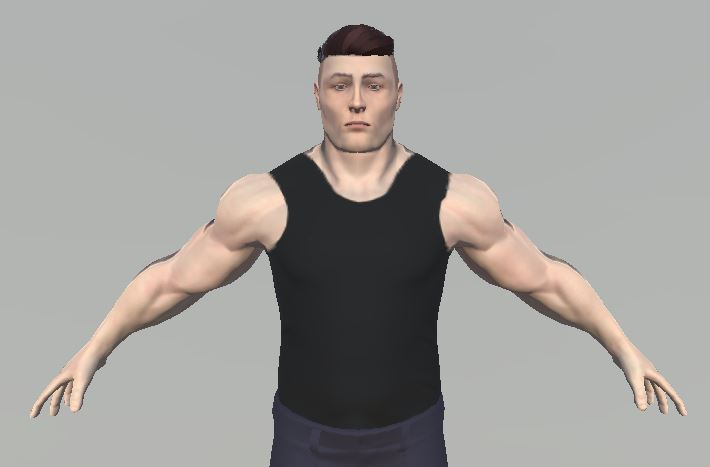
\includegraphics[width=\linewidth]{Images/Males/6.JPG}
\endminipage\hfill
\minipage{0.5\textwidth}
  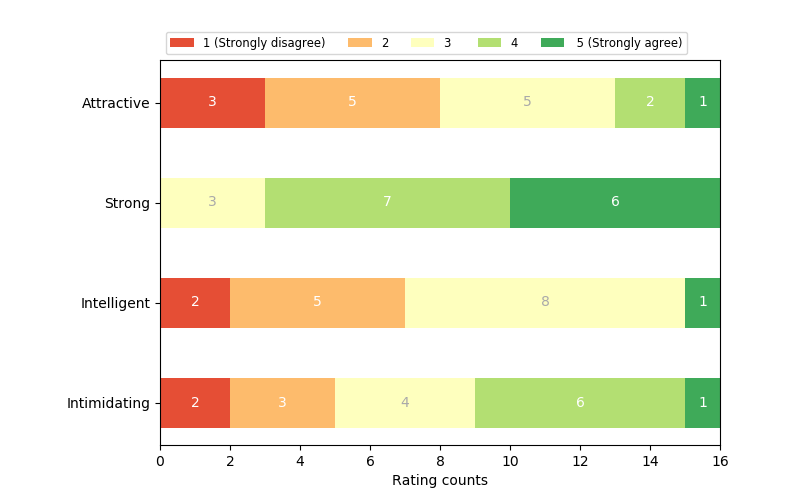
\includegraphics[width=\linewidth]{Survey/MRatings/avatar_m6.png}
\endminipage\hfill
\caption{Male 6 thumbnail and ratings.}
\end{figure}

\begin{figure}[H]
\minipage{0.5\textwidth}
  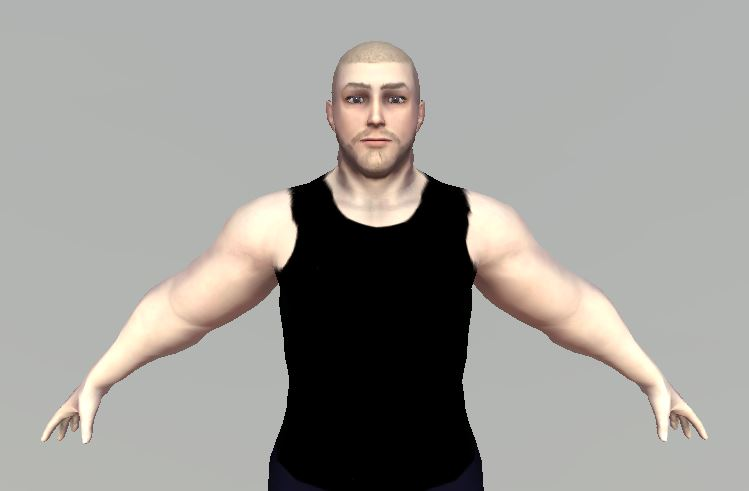
\includegraphics[width=\linewidth]{Images/Males/7.JPG}
\endminipage\hfill
\minipage{0.5\textwidth}
  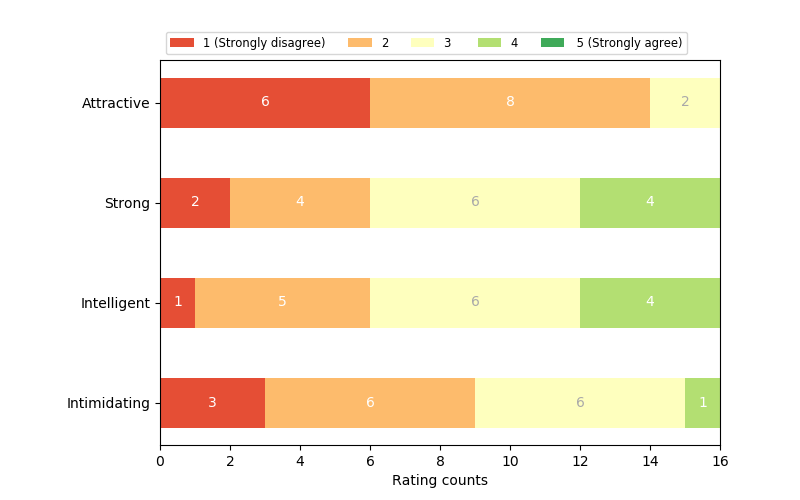
\includegraphics[width=\linewidth]{Survey/MRatings/avatar_m7.png}
\endminipage\hfill
\caption{Male 7 thumbnail and ratings.}
\end{figure}


\begin{figure}[H]
\minipage{0.5\textwidth}
  \includegraphics[width=\linewidth]{Images/Males/8.JPG}
\endminipage\hfill
\minipage{0.5\textwidth}
  \includegraphics[width=\linewidth]{Survey/MRatings/avatar_m8.png}
\endminipage\hfill
\caption{Male 8 thumbnail and ratings.}
\end{figure}

\begin{figure}[H]
\minipage{0.5\textwidth}
  \includegraphics[width=\linewidth]{Images/Males/9.JPG}
\endminipage\hfill
\minipage{0.5\textwidth}
  \includegraphics[width=\linewidth]{Survey/MRatings/avatar_m9.png}
\endminipage\hfill
\caption{Male 9 thumbnail and ratings.}
\end{figure}


\begin{figure}[H]
\minipage{0.5\textwidth}
  \includegraphics[width=\linewidth]{Images/Males/10.JPG}
\endminipage\hfill
\minipage{0.5\textwidth}
  \includegraphics[width=\linewidth]{Survey/MRatings/avatar_m10.png}
\endminipage\hfill
\caption{Male 10 thumbnail and ratings.}
\end{figure}

\begin{figure}[H]
\minipage{0.5\textwidth}
  \includegraphics[width=\linewidth]{Images/Males/10.JPG}
\endminipage\hfill
\minipage{0.5\textwidth}
  \includegraphics[width=\linewidth]{Survey/MRatings/avatar_m10.png}
\endminipage\hfill
\caption{Male 10 thumbnail and ratings.}
\end{figure}

\begin{figure}[H]
\minipage{0.5\textwidth}
  \includegraphics[width=\linewidth]{Images/Males/11.JPG}
\endminipage\hfill
\minipage{0.5\textwidth}
  \includegraphics[width=\linewidth]{Survey/MRatings/avatar_m11.png}
\endminipage\hfill
\caption{Male 11 thumbnail and ratings.}
\end{figure}

\begin{figure}[H]
\minipage{0.5\textwidth}
  \includegraphics[width=\linewidth]{Images/Males/12.JPG}
\endminipage\hfill
\minipage{0.5\textwidth}
  \includegraphics[width=\linewidth]{Survey/MRatings/avatar_m12.png}
\endminipage\hfill
\caption{Male 12 thumbnail and ratings.}
\end{figure}


\begin{figure}[H]
\minipage{0.5\textwidth}
  \includegraphics[width=\linewidth]{Images/Males/13.JPG}
\endminipage\hfill
\minipage{0.5\textwidth}
  \includegraphics[width=\linewidth]{Survey/MRatings/avatar_m13.png}
\endminipage\hfill
\caption{Male 13 thumbnail and ratings.}
\end{figure}

\begin{figure}[H]
\minipage{0.5\textwidth}
  \includegraphics[width=\linewidth]{Images/Males/14.JPG}
\endminipage\hfill
\minipage{0.5\textwidth}
  \includegraphics[width=\linewidth]{Survey/MRatings/avatar_m14.png}
\endminipage\hfill
\caption{Male 14 thumbnail and ratings.}
\end{figure}


\begin{figure}[H]
\minipage{0.5\textwidth}
  \includegraphics[width=\linewidth]{Images/Males/15.JPG}
\endminipage\hfill
\minipage{0.5\textwidth}
  \includegraphics[width=\linewidth]{Survey/MRatings/avatar_m15.png}
\endminipage\hfill
\caption{Male 15 thumbnail and ratings.}
\end{figure}

\begin{figure}[H]
\minipage{0.5\textwidth}
  \includegraphics[width=\linewidth]{Images/Males/16.JPG}
\endminipage\hfill
\minipage{0.5\textwidth}
  \includegraphics[width=\linewidth]{Survey/MRatings/avatar_m16.png}
\endminipage\hfill
\caption{Male 16 thumbnail and ratings.}
\end{figure}

\begin{figure}[H]
\minipage{0.5\textwidth}
  \includegraphics[width=\linewidth]{Images/Males/17.JPG}
\endminipage\hfill
\minipage{0.5\textwidth}
  \includegraphics[width=\linewidth]{Survey/MRatings/avatar_m17.png}
\endminipage\hfill
\caption{Male 17 thumbnail and ratings.}
\end{figure}


\begin{figure}[H]
\minipage{0.5\textwidth}
  \includegraphics[width=\linewidth]{Images/Males/18.JPG}
\endminipage\hfill
\minipage{0.5\textwidth}
  \includegraphics[width=\linewidth]{Survey/MRatings/avatar_m18.png}
\endminipage\hfill
\caption{Male 18 thumbnail and ratings.}
\end{figure}

\subsection{Recruiting Poster}
\label{subsection:poster}

\begin{figure}[H]
\centering
\minipage{0.5\textwidth}
  \includegraphics[width=\linewidth]{Images/poster.png}
\endminipage
\end{figure}
